%\title{emnlp 2017 instructions}
% File emnlp2017.tex
%

\documentclass[11pt,letterpaper]{article}
\usepackage{emnlp2017}
\usepackage{times}
\usepackage{latexsym}
\usepackage{url}
\usepackage{multirow}
\usepackage{multicol}
\usepackage{array}
\usepackage{graphicx}
\usepackage{footnote}
\makesavenoteenv{table}
\usepackage{amsmath, bm}
\usepackage[english,american]{babel}
\usepackage{color}

\newcommand\FIXME[1]{\textcolor{red}{FIX:}\textcolor{red}{#1}}


% Uncomment this line for the final submission:
%\emnlpfinalcopy

%  Enter the EMNLP Paper ID here:
\def\emnlppaperid{***}

% To expand the titlebox for more authors, uncomment
% below and set accordingly.
% \addtolength\titlebox{.5in}

\newcommand\BibTeX{B{\sc ib}\TeX}

\title{Event Extraction without Human-annotated Text}
\author{Siddharth Patwardhan \and Preethi Raghavan \\
  {\tt publication@emnlp2017.net}}

\date{}

\begin{document}

\maketitle

\begin{abstract}
Existing event extraction systems are typically investigated in the supervised
learning paradigm. The effectiveness of these systems heavily relies on the quality of
expert-annotated datasets which still require a costly and time-consuming process to construct.
 As a result, the built datasets
often only cover a limited variety of event types, making the
learned event extractor hard to generalize. In this paper, we address the problem
of automatically building event extractors for rich event types with little expert involvement.
We achieve this by employing distant supervision to automatically create event annotations from
unlabelled data using structured knowledge bases. We then propose a novel
neural network model with ILP-based inference, committing to detecting events of various types and extracting
their corresponding arguments involved.
We evaluate our approach by automatically collecting training data for many event types from Freebase, where
our proposed extraction model is designed to identify both typed event mentions and typed arguments. Both automatic and
manual evaluations demonstrate that it is possible to learn to effectively extract
various events without human-annotated training data.

%
%and rely on expert-annotated datasets, with limited event types.
%%such as ACE and ERE event extraction frameworks.
%However, designing and constructing these
%high-quality corpora, usually with limited size and coverage of event types,  is costly, which
%makes learned extractors hard to generalize.  With the essence of distant supervision,
%%Inspired by some Freebase schemas which share similar structures with ACE event templates,
%we investigate the possibilities of automatic construction of training data for various event types
%with the help of structured knowledge bases.
%the following problems in this paper: can we generate a feasible dataset for event extraction with Freebase automatically and is it possible to extract events on this dataset.
%We first propose four hypotheses based on our observation and produce our dataset accordingly. Then,
%We further propose a novel neural network with ILP-based post inference, committing to
%handling two challenges in event extraction: multi-type events and multi-word arguments.
%Both automatic and manual evaluations demonstrate that it is possible to learn to extract various  events, according to existing knowledge bases, without human-annotated training data.
\end{abstract}

\section{Introduction}
%Automatically extracting events from natural text remains a challenging task in information extraction. Among diverse types of event extraction systems, the extraction task proposed by Automatic Content Extraction (ACE) \cite{doddington2004automatic} is the most popular framework, which defines two main terminologies: \textbf{trigger} and \textbf{argument}. The former is the word that most clearly expresses the occurrence of an event. The latter is a phrase that serves as a participant or attribute with a specific role in an event.
%
%However, constructing training data for ACE task is expensive. First, linguists are required to summarize a large amount of text to elaborately design templates about potential arguments for each event type. Second, rules should be explicitly stated to guide annotators. In spite of detailed guidelines, there is still disagreement among human annotators about what should (not) be regarded as triggers/arguments.
%For example, can a prepositional phrase or a portion of a word trigger an event, e.g., \textit{in prison} triggers an \emph{arrest} event,
%or, \textit{ex} in \textit{ex-husband} triggers a \emph{divorce} event?
%Besides, ACE event extraction systems have two major limitations:   single-token trigger labeling, and one type for one event.

Event extraction, as represented by the Automatic Content Extraction (ACE) task, is a key enabling
technique for many natural language processing (NLP) applications.  Current event extractors are typically built through applying supervised learning to learn over labelled datasets. This means that the performance of event extraction systems highly dependent on the quality of the training datasets.

Constructing high-quality training data for event extraction is, however, an expensive and error-prone process\FIXME{\cite{}}. This requires the involvement of linguists to design annotation templates and rules, and the employment of annotators to manually label data. To scale up event extraction, we need to reduce expert involvement.
In addition to the extensive human involvement, existing event extraction systems have two major drawbacks -- they can only handle (1)  single-token triggers\footnote{In the ACE task, a trigger is the word that most clearly expresses the occurrence of an event.} and (2) and scenarios where  each event is merely associated with a single type.
To make event extractors practical, we need to support situations where the trigger annotations are unavailable or one event is associated with multiple types.


%The aforementioned drawbacks of ACE event extraction systems motivate us to
%It would be interesting to see (1) can we automatically build a dataset for event extraction without experts involved?
%and (2) can we have an event extractor that handles more realistic scenarios, e.g.,  when trigger annotations are unavailable, or events with more than one type.


This paper presents a novel approach for automatic training data generation, specifically targeting event extraction. Our approach advances prior work\FIXME{\cite{}} in two aspects: (1) it does not rely on expert-annotated texts (hence it reduces expert involvement) and (2) supports multi-typed events. The former is achieved by employing distant supervision to automatically annotate event structures from plain text, using information extracted from existing structured knowledge bases such as Freebase. The later is achieved by using a novel neural network model with ILP-based inference to extract multiple event types without relying on explicit trigger annotations.


Our first insight is that structured knowledge bases (\KB) typically organize
complex structured information in tables; and these tables often share similar structures with ACE event definitions, i.e. a particular entry of such tables usually implies the occurrence of certain events.
Recent studies \cite{mintz2009distant,zeng2015distant} have demonstrated the effectiveness of \KB as distant supervision (\DS) for binary relation extraction. In this paper, we aim to extend \DS to extract events of n-ary relations and multiple arguments (rather than just binary
relation). One of the hurdles for doing this is the lacking of explicit trigger information in existing \KB. 
Our solution to the problem is to use a group of \textbf{key arguments} rather than explicit triggers to capture a particular event. For example, we can use ``\emph{spouse}'' as the key argument to identify ``\emph{marriage}'' events.


%However, there are two major challenges when leveraging KB to event extraction: first, event structures are more complex than binary relations. They can be represented as $\langle event\_type, argument_1, \ldots, argument_n\rangle$, which are n-ary relations with various numbers of arguments. Second, there is no explicit trigger information in any existing knowledge base.
%However, we find that for a particular event type, there is a group of \textbf{key arguments} which together can imply an event instead of explicit triggers. For example, ``\emph{spouse}'' is the key argument of ``\emph{marriage}'' events, while ``\emph{location of ceremony}'' is too generic to become a key argument. Therefore, we put forward a distant supervision approach to event extraction: a sentence that contains all key arguments of an event is likely to express that event in some way. To explore the sets of key arguments, we investigate different hypotheses for better data quality and quantity.

% Therefore, to explore the distant supervision (\texttt{DS}) assumption in event extraction, we investigate different hypotheses for better data quality and quantity. Among them, the vital one is that, for a particular event type, there is a group of \textbf{key arguments} which together can imply an event instead of explicit triggers.


%We utilize Freebase as our knowledge base and Wikipedia articles as text for data generation as a major source of Freebase is the tabular data from Wikipedia \cite{mintz2009distant}.
% According to Mintz et al. \shortcite{mintz2009distant}, because a major source of Freebase is the tabular data from Wikipedia, making it a natural fit with Freebase.
%Figure~\ref{fig:3} illustrates examples of sentences annotated by our algorithm.

Our second innovation is that unlike previous studies which focus on tasks defined by ACE evaluation framework \cite{ahn2006stages,li2013joint,chen2015event,nguyen2016joint}, we propose a novel event extraction paradigm with key arguments to characterize an event type. We consider event extraction as two sequence labeling subtasks, namely event detection and argument detection. Inspired by neural network models in sequence labeling tasks \cite{huang2015bidirectional,lample2016neural}, we utilize LSTM-CRF models to label key arguments and non-key arguments in the each sentence separately. However, event structures are not simple sequences and there are strong dependencies among key arguments. We therefore reformulate the hypotheses as constraints, and apply linear integer programming to output multiple optimal label sequences to capture multi-type events.

We evaluate our approach by applying it to automatically collect training data with multiple event types using Freebase. 
We use the proposed extraction model to identify both typed event mentions and typed arguments. Our experitmental
results on both automatic and
manual evaluations demonstrate that our approach can effectively extract
various events without human-annotated training data. \FIXME{quantified numbers?}


%In this paper, we exploit existing structured knowledge bases, e.g., Freebase, as distant supervision to automatically annotate event structures from plain text without human annotations. We further propose a novel event extraction paradigm that harnesses key arguments to imply certain event types without explicit trigger annotations. We present an LSTM-CRF model with post inference to extract both Freebase-style events as well as multi-type event mentions on the generated dataset, which is demonstrated effective by both manual and automatic evaluations.

\section{The Event Extraction Task}
%\subsection{Event Definition}
% 给出相关术语的定义,subsection名字起得对吗?
Event extraction aims to detect the occurrence of events with specific types and extract their typed participants or attributes from text. We clarify the following terminologies within our work:
\begin{itemize}
	\item \textbf{Event mention}: a phrase or sentence within which an event is described, including its type and arguments.
	\item \textbf{Argument}: an entity mention, temporal expression or value that is involved in an event, with specific roles.
	\item \textbf{Key argument}: the argument that plays an important role in one event, and helps to distinguish with other events. % 要不要举例说明什么是key argument?这里再举例会不会和introduction里面的举例重复?
	% 没有地方的时候,argument role可以删掉(我看别人ACE定义的时候都讲了这个就先放上来了)
	%\item \textbf{Argument role}: the relationship between an event and its involved argument. 
\end{itemize}

\subsection{Indirect Supervision for Event}%{Tabular Data}
% 缺一句连接的话?
We first utilize Freebase~\cite{bollacker2008freebase} as a source of supervision to guide our data construction, %the structured knowledge base.
% and there are three basics concepts: \emph{instance}, \emph{type} and \emph{property}. \emph{Instances} are entries in Freebase. \emph{Types} are different perspectives of \emph{instances}. 
where \textbf{\emph{Compound Value Type}} (CVT) is a special type to represent complex structured data % where entries are described 
with multiple \emph{properties}, usually organized in a table. Some CVT schemas indeed imply certain events, e.g., \emph{business.acquisition},
% \emph{military.military\_service} and \emph{people.marriage}, 
and closely resemble to event structures, where CVT properties can be treated as event arguments\footnote{
Therefore, we also use the term ``argument'' to refer to CVT property in the rest of paper.}. % 直接在这里说CVT property其实就是argument,后面描述的时候不会太咯嗦
As shown in Figure~\ref{fig:3}, the properties of CVT \emph{business.acquisition} actually can be used to label arguments of the events mentioned in S1 and S2. 
We use the Freebase copy of 2013-06,  %version of Berant et al. \shortcite{berant2013semantic}, 
containing 1010 CVTs. After manually filtering out those % CVTs that 
describing Freebase structure or irrelevant to events, %(e.g., \emph{food.recipe\_ingredient})
 we obtain 24 CVTs with around 280 million instances.

\begin{figure}[h]
	\centering
	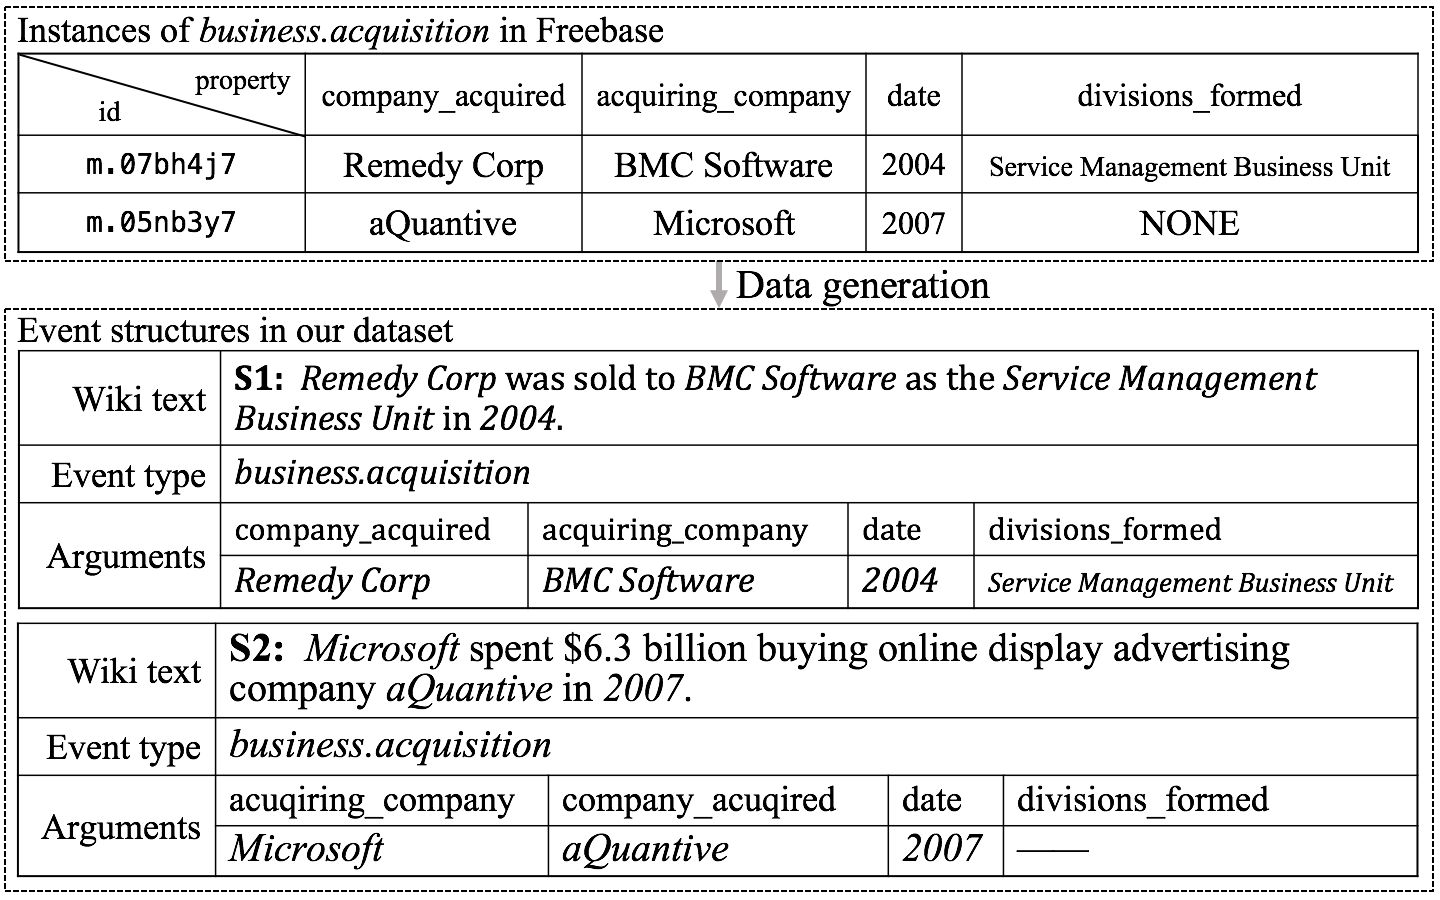
\includegraphics[width=.48\textwidth]{temp}
	\caption{Examples of a CVT table in Freebase, and labeled sentences in our dataset. \emph{Company\_acquired}, \emph{acquiring\_company} and \emph{date} are key arguments in \emph{business.acquisition}. \label{fig:3}}
\end{figure}

Besides structured knowledge base, tables or lists that are used to sum up certain activities or occasions could be considered as a source of supervision for event extraction, as well. 
We thus investigate tables collected from Wikipedia pages, potentially referring to three types: winning of the Olympics, music and film awards, mergers and acquisitions\footnote{For example, \url{https://en.wikipedia.org/wiki/List_of_mergers_and_acquisitions_by_IBM}}.

\subsection{Dataset Construction\label{datagen}} 
% 在哪里说其实 property 在后面就是 argument 了
Here, we employ the event-related entries of Freebase CVT tables to illustrate how to automatically annotate event mentions in Wikipedia's articles, with the essence of distant supervision (\textbf{\texttt{DS}}): \textit{A sentence that contains \textbf{all key arguments} of an entry in an event table (e.g., CVT table) is likely to express that event}.
%\begin{quote}
%	\textbf{\texttt{DS}}: A sentence that contains all key arguments of an entry in an event table (e.g., CVT table) is likely to express that event in some way.
%\end{quote}
We will then label this sentence as a mention of this CVT event, and the words or phrases that match this entry's properties as the involved arguments, with the roles specified by their corresponding property names. 

We regard a sentence as \emph{positive} when it mentions the occurrence of an event, or  \emph{negative} otherwise. 
For example, S1 and S2 are positive examples with their arguments in italics and underlined (also shown in Figure~\ref{fig:3}), while S3 and S4 are negative.
%
\begin{quote}
	\textbf{S1}: \underline{\emph{Remedy Corp}} was sold to \underline{\emph{BMC Software}} as the \underline{\emph{Service}} \underline{\emph{Management Business Unit}} in \underline{\emph{2004}}.
\end{quote}
\begin{quote}
\textbf{S2}: \underline{\emph{Microsoft}} spent \$6.3 billion buying online display advertising company \underline{\emph{aQuantive}} in \underline{\emph{2007}}.
\end{quote}
\begin{quote}
\textbf{S3}: Microsoft hopes aQuantive's Brian McAndrews can outfox Google.
\end{quote}
\begin{quote}
\textbf{S4}: On April 29th, Elizabeth II and Prince Philip witnessed the marriage of Prince William.
\end{quote}

The selection strategy for key arguments for a given event type is based on two criteria: (1) \emph{Key arguments should have high importance value}; (2) \emph{Key arguments should include time-related arguments}.

% \paragraph{H1: Positive sentences should contain all properties}

% For example, S1 contains all the properties of instance $m.07bh4j7$ with a CVT type \emph{business.acquisition}, we thus consider S1 as a positive sample implying an event about \emph{business.acquisition}, and \emph{BMC Software}, \emph{Remedy Corp}, \emph{Service Management Business Unit} and \emph{2004} will be labeled as the arguments that play the role of \emph{acquiring\_company}, \emph{company\_acquired}, \emph{divisions\_formed}, and \emph{date} in this event, respectively.
% However, in practice, we realize that \emph{H1} is too strict that excludes a great many positive sentences like S2. 
% In practice, we find that \emph{H1} is too strict to include many positive sentences like S2. 
% We thus relax \emph{H1} by replacing \textbf{all properties} with \textbf{all key properties}. 

The \emph{Importance value} of an argument $arg$ (e.g., \emph{date}) to its event type $cvt$ (e.g., \emph{business.acquisition}) can be defined as:
\begin{equation}
	I_{cvt, arg} = log \frac{count(cvt, arg)}{count(cvt) \times count(arg)} 
\end{equation}
where $count(cvt)$ is the number of instances of type $cvt$, $count(arg)$ is the number of times $arg$ appearing in all CVT types, and $count(cvt, arg)$ is the number of $cvt$ instances that contain $arg$.

% We discover that for many CVTs, their key properties do not take into account time property. 
% time-related argument叫得对吗?本来的想说的是,取值为时间的argument
Although time-related arguments are often missing in the currently imperfect KBs, 
they are indeed crucial to indicate the actual occurrence of an event, e.g., S3, containing \emph{Microsoft} as \emph{acquiring\_company} and \emph{aQuantive} as \emph{company\_acquired} but without time-related arguments, will be mistakenly considered as a positive sample for event \emph{business.accquisition}.
% while contain all key properties of an instance, resulting in mistaking \emph{Microsoft} for \emph{acquiring\_company}, and \emph{aQuantive} for \emph{company\_acquired}. 
% By adding \emph{date} to the set of key properties, S3 will be filtered. 

Intuitively, two arguments involving in the same event mention are likely to be closer within the syntactic structure.
% , which will help to eliminate negative samples. 
In Figure~\ref{fig:2}, both \emph{Prince Philip} and \emph{marriage} can be matched as key arguments in a \textit{people.marriage} entry, but are far from each other on the dependency parse tree, thus S4 should be labeled as negative.
% We thus set the maximum distance between two key arguments as 2 empirically.
%, i.e., for a candidate sentence, if a pair of key arguments violates this constraint, it is supposed to be negative. 
% Given the dependency parsing tree in Figure~\ref{fig:2}, S4 is negative because the distance between \emph{Prince Philip} and \emph{marriage} is 3.

\begin{figure}
\centering
	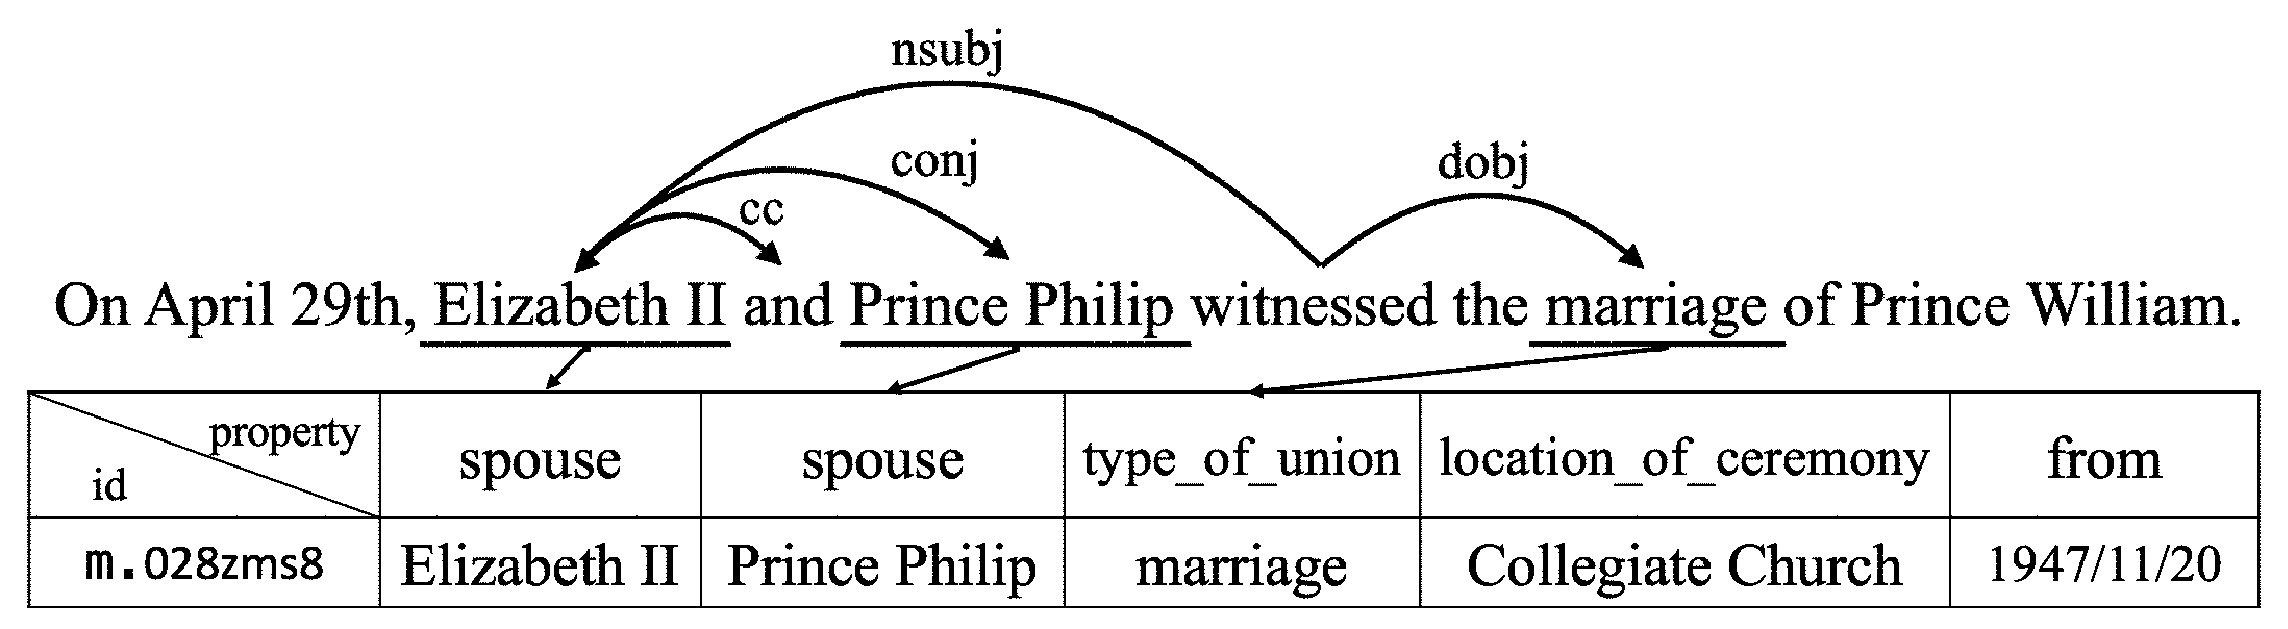
\includegraphics[width=.47\textwidth]{deppath3.eps}
	\caption{The dependency tree of S4, which partially matches an entry of \emph{people.marriage}. \label{fig:2}}
\end{figure}

We conduct a series of manual evaluations on the quantity and quality of the datasets produced by different strategies (see Sec~\ref{sec:evalhypo}), and 
% following strategy produces the best dataset, thus serves as 
our final strategy is: 
for each CVT, we first sort all its arguments in descending order by their importance values, and select the top half arguments as key arguments. 
We then include the time-related argument with highest importance value as a supplementary key argument. 
Finally, we eliminate sentences in which the dependency distances between any two key arguments are greater than 2.

% 好像没地方了,先不写了
% \begin{table}
% \centering
% \small
% \begin{tabular}{|l|l|} \hline
% CVT & Key arguments \\ \hline
% award.award\_honor & award\_winner, award, \ldots, year \\ \hline
% film.performance & actor, film, character \\ \hline
% education.education & institution, student, end\_date \\ \hline
% business.employment\_tenure & company, title, person, from \\ \hline
% \end{tabular}
% \caption{Examples of key arguments of four CVTs.\label{tab:5}}
% \end{table}

%\subsection{Our Task}
%Previous event extraction systems rely on explicit trigger identification to detect the occurrence of an event, 
%which is then used to decide its event type and label its arguments.
%In our automatically collected dataset, where human-labeled event triggers are unavailable, we argue that \textbf{key arguments} can play the same role as explicit event triggers. 
%We thus treat the event extraction as a pipeline of the following two steps: 
%\begin{itemize}
%	\item \textbf{Event detection}: to identify key arguments in a sentence. If a sentence contains \textbf{all key arguments} of a specific event type, it will be considered to imply an event mention of this specified type. 
%	\item \textbf{Argument detection}: to identify other non-key arguments for each event in the sentence.
%\end{itemize}
%
%Take S1 as an example, in event detection, \emph{Remedy Corp}, \emph{BMC Software}, and \emph{2004} could be identified as \emph{company\_acquired}, \emph{acquiring\_company}, and \emph{date}, respectively, indicating that S1 may mention a \emph{business.acquisition} event. 
%During argument detection, \emph{Service Management Business Unit} should be identified as \emph{divisions\_formed}, 
%which, together with the detected key arguments, form a full mention for a \emph{business.acquisition} event.  

\section{Our Approach}
%\subsection{Our Task}
Previous event extraction systems mainly rely on explicit trigger identification to detect the occurrence of an event, 
which is then used to decide its event type and label its arguments.
In our automatically collected dataset, where human-labeled event triggers are unavailable, we argue that \textbf{key arguments} can play the same role as explicit event triggers. 
We thus treat the event extraction as a pipeline of the following two steps: 
\begin{itemize}
	\item \textbf{Event detection}: to identify key arguments in a sentence. If a sentence contains \textbf{all key arguments} of a specific event type, it will be considered to imply an event mention of this specified type. 
	\item \textbf{Argument detection}: to identify other non-key arguments for each event in the sentence.
\end{itemize}
%
Take S1 as an example, in event detection, \emph{Remedy Corp}, \emph{BMC Software}, and \emph{2004} could be identified as \emph{company\_acquired}, \emph{acquiring\_company}, and \emph{date}, respectively, indicating that S1 may mention a \emph{business.acquisition} event. 
During argument detection, \emph{Service Management Business Unit} should be identified as \emph{divisions\_formed}, 
which, together with the detected key arguments, form a full mention for a \emph{business.acquisition} event.  

\subsection{Event Detection \label{evede}}
%Before presenting our model, 
%Our event detector is an BLSTM-CRF model with ILP-based inference.  
%We first present our solution for multi-words arguments, and then introduce each component in our model.
%BLSTM-CRF-ILP$_{multi}$ model, from bottom to top.

% \vspace{-.8em}
%\paragraph{Tagging scheme}
68\%  of  arguments in our dataset consist of more than one word. We thus formulate each subtask in a sequence labeling paradigm rather than word-level classifications. Each word in the given sentence is tagged with the \texttt{BIO} scheme, where each token is labeled as \texttt{B-role} if it is the beginning of an event argument with its corresponding role \texttt{role}, or \texttt{I-role} if it is inside an argument, or \texttt{O} otherwise.  We accordingly propose a novel BLSTM-CRF model with ILP-based inference to detect and organize key arguments.

% \vspace{-.7em}
\paragraph{BLSTM}
Long Short-Term Memory Network (LSTM)~\cite{hochreiter1997long} is a natural fit for sequence labeling, which maintains a memory based on historical contextual information. Formally, given a sentence $\bm{w} = \{w_1, w_2, \dots, w_n\}$ of length $n$, we use $\textbf{x}_t$ to represent feature vector, e.g., word embeddings, corresponding to the $t$-th word $w_t$. 
At each time $t$, a forward LSTM layer takes $\textbf{x}_t$ as input and computes the output vector $\overrightarrow{\textbf{h}}_t$ of the past context, while a backward LSTM layer reads the same sentence in reverse and outputs $\overleftarrow{\textbf{h}}_t$ given the future context. We concatenate these two vectors to form the output vector of BLSTM, which is fed into a softmax layer to estimate a probability distribution over all possible labels.

% \vspace{-.8em}
\paragraph{CRF}
A straightforward way to find the label sequence for given sentence is to choose the 
best label for each word individually according to the BLSTM output.  
%with maximum probability by LSTM as the prediction for each word. 
However, this greedy strategy ignores the dependencies between labels, thus can not guarantee the best sequence.  %this independent labeling strategy 
%is limited especially when there are strong dependencies and constraints between labels. 
%To model the correlations between labels, 
Therefore, we introduce a CRF layer over the BLSTM output, which is admittedly effective in various sequence labeling tasks~\cite{collobert2011natural,huang2015bidirectional}. %, such as POS tagging and NER .

We consider $\textbf{P}$ to be a matrix of confidence scores output by BLSTM, and the element $\textbf{P}_{i,j}$ of the matrix denotes the probability of the label $j$ for the $i$-th word in a sentence. The CRF layer takes a transition matrix $\textbf{A}$ as parameter, where $\textbf{A}_{i,j}$ represents the score of a transition from label $i$ to label $j$. The score of a sentence $\bm{w}$ along with a path of labels $\bm{y} = \{y_1, y_2, \ldots, y_n\}$ is measured by the sum of BLSTM outputs and transition scores: 
\begin{equation}
	score(\bm{w}, \bm{y}) = \sum\limits_{i=0}^n\textbf{P}_{i, y_i} + \sum\limits_{i=1}^n\textbf{A}_{y_i, y_{i+1}},
\end{equation}
During test, given a sentence $\bm{w}$, we adopt the Viterbi algorithm~\cite{rabiner1989tutorial} to find the optimal label sequence with the maximum score among all possible label sequences.

% \vspace{-.8em}
\paragraph{ILP-based Post Inference}
Basically, event detection is a structure prediction problem, while the output sequences of BLSTM-CRF do not necessarily satisfy the structural constraints. For instance, regardless of how many key arguments are correctly identified by BLSTM-CRF, if there is one key argument missing, this detection should be considered as failed. 

We thus propose to apply Integer Linear Programming (ILP) to further globally optimize the BLSTM-CRF output  to produce the best label sequence.
Formally, let $\mathcal{L}$ be the set of possible argument labels. For each word $w_i$ in the sentence $\bm{w}$ and a pair of labels $ \langle l, l' \rangle \in \mathcal{L} \times \mathcal{L}$, we create a binary variable ${v_{i,l,l'} \in \{0, 1\}}$, denoting whether or not the $i$-th word $w_i$ is tagged as label $l$ and its following word $w_{i+1}$ is tagged as label $l'$ at the same time. The objective of ILP is to maximize the overall score of the variables as:
\begin{displaymath}
	\sum\nolimits_{i, l, l'}v_{i,l,l'} * (\textbf{P}_{i,l}+\textbf{A}_{l,l'}) .
\end{displaymath}
where we consider the following four constraints:

\textbf{C1}: Each word should be and only be annotated with one label, i.e.:
\begin{equation}
	\sum\nolimits_{l,l'}v_{i,l,l'}=1
\end{equation}

\textbf{C2}: If the value of $v_{i,l,l'}$ is $1$, then there has to be a label $l^*$ that will make $v_{i+1,l',l^*}$ equal to $1$, i.e.:
\begin{equation}
	v_{i,l,l'} = \sum\nolimits_{l^*}v_{i+1,l',l^*}
\end{equation}

\textbf{C3}: If the current label is \texttt{I-arg}, then its previous label must be \texttt{B-arg} or \texttt{I-arg}, i.e.:
\begin{equation}
	v_{i,\texttt{I-arg},l'} = v_{i-1,\texttt{B-arg},\texttt{I-arg}} + v_{i-1, \texttt{I-arg}, \texttt{I-arg}}
\end{equation}

\textbf{C4}: For a specific event type, all its key arguments should co-occur in the sentence, or none of them appears in the resulting sequence. For any pair of key arguments $arg_1$ and $arg_2$ with respect to the same event type, the variables related to them are subject to:
\begin{equation}
	\sum\nolimits_{i,l'}{v_{i,\texttt{B-arg}_1,l'}} \leq n * \sum\nolimits_{j,l^*}{v_{j,\texttt{B-arg}_2,l^*}}
\end{equation}
where $n$ is the length of the sentence.

In order to address the multi-type event mention issue, we allow our ILP solver to output multiple optimal sequences. 
Specifically, after our model outputs the best sequence $\bm{s}^t$ at time $t$, we remove the previously best solutions 
%Formally, let $\bm{s}^t=\{l_1^t, l_2^t, \ldots, l_n^t\}$ be the sequence produced at iteration $t$. During each iteration $t$, 
 $\{\bm{s}^1, \ldots, \bm{s}^{t}\}$ from the solution space, and re-run our solver to obtain the next optimal sequences $\bm{s}^{t+1}$. 
We repeat the optimization procedure until the difference between the scores of $\bm{s}^1$ and $\bm{s}^T$ is greater 
than a threshold $\lambda$, and consider all solutions $\{\bm{s}^1, \bm{s}^2, \ldots, \bm{s}^{T-1}\}$ as the optimal label sequences. 
We use Gurobi~\cite{gurobi} as our ILP solver and set $\lambda=0.05 \times n$, which averagely produce~1.04 optimal sequences for each sentence. 

\subsection{Argument Detection}
After event detection, a sentence will be classified into different event types, and labeled with its corresponding key arguments. 
%The next step is argument detection, which 
Next, we will identify the remaining non-key arguments in the sentence. 

We adopt the same BLSTM-CRF architecture (in Sec~\ref{evede}) for argument detection, where we encode the event label (output of event detection) of each word into a key-argument feature vector through a look-up table, and concatenate it with the original word embedding as the input to the new BLSTM-CRF. Note that we do not need post inference here.
\section{Experiments}
\subsection{Experimental Setup}
%\textbf{Dataset and Evaluation Methodology}. 
We use Freebase and the English Wikipedia dump of 2016-11-20, to construct our dataset. Statistics for the generated dataset is shown in Table~\ref{statistics}. Note that all sentences in the dataset are positive. 
\begin{table}
\small
\centering
\begin{tabular}{|l|c|c|c|} \hline
& Train & Dev & Test \\ \hline
\emph{\#Sent.} & 4800 & 1200 & 1180 \\ \hline
\emph{\#Eve.} & 4918 & 1247 & 1229 \\ \hline
\emph{\#Arg.} & 17274 & 4318 & 4248 \\ \hline
\emph{\%Multi\_Eve.} & 3.0 & 3.2 & 3.1 \\ \hline
% \emph{\%Multi\_Arg.} & 67.4 & 67.0 & 67.9 \\ \hline
\end{tabular}	
\caption{Statistics for the generated dataset. \emph{\#Sent.} is the number of sentences, \emph{\#Eve.} is the number of event mentions, and \emph{\#Arg.} is the number of event arguments. \emph{\%Multi\_Eve.} is the ratio of multi-type events.
%, and \emph{\%Multi\_Arg.} is the ratio of multi-word arguments.
\label{statistics}}
\end{table}
% containing 7,180 sentences, containing 7,394 events and 25,840 arguments. We then randomly select 4,800 sentences for training and 1,180 sentences as test set, and the rest 1,200 sentences for validation. 
We first manually evaluate the quality of our test set and then regard the automatically generated data as gold standard and evaluate our model accordingly. Next, we manually evaluate a subset of events detected by our model and analyze the differences with regards to the automatic evaluation. Finally, we conduct evaluation on a smaller dataset annotated by tables crawled from Wikipedia's pages. 

\paragraph{Evaluation Measures} We evaluate our models in terms of precision (P), recall (R), and F-measure (F) for each subtask. These performance metrics are computed according to the following standards of correctness: 
For \emph{event type classification}, an event is correctly classified if its reference sentence contains all key arguments of this event type. 
For \emph{argument detection}, an argument is correctly detected if its offsets, role, and related event type exactly match the reference argument within the same sentence. 
For \emph{event detection}, an event is correctly detected if its type and all its key arguments match a reference event within the same sentence.

\paragraph{Training} All hyper-parameters are tuned on the development set. In event detection, we set the size of word embeddings to 200, the size of LSTM layer to 100. In argument detection, we use the same size of word embedding, while the size of LSTM layer is 150, and the size of key argument embedding is 50. Word embeddings are pre-trained using skip-gram word2vec~\cite{mikolov2013distributed} on English Wikipedia pages and fine tuned during training. To mitigate overfitting, we apply a dropout rate of 0.5 on both the input and output layers.

\subsection{Dataset Evaluation}\label{sec:evalhypo}
To investigate the possibility of automatically constructing training data for event extraction, we evaluate five datasets that utilize  following strategies to determine key arguments and collect positive sentences from Wikipedia pages: (1) \emph{ALL} means regarding all arguments as key arguments; (2) \emph{IMP} means selecting the top half arguments with high importance value as key arguments; (3) \emph{IMP\&TIME} means adding a time-related argument with highest importance value to the set of key arguments generated by \emph{IMP}; (4) \emph{DIS} means eliminating sentence where dependency distances between any two key arguments are greater than 2. We randomly select 100 sentences in each dataset, and annotators are asked to determine whether each sentence implies a given event.

% 怎么介绍Strategy比较省地方?
\begin{table}[h]
\small
\centering
\begin{tabular}{|c|l|c|c|c|} \hline
	No. & Selection strategy & Dataset & Type & Pos \\ \hline
	S1 & \emph{ALL} & 203 & 9 & 98 \\ \hline
	S2 & \emph{IMP} & 108K & 24 & 22 \\ \hline
	S3 & \emph{IMP} + \emph{DIS} & 12K & 24 & 37 \\ \hline
	S4 & \emph{IMP\&TIME} & 9241 & 24 & 81 \\ \hline
	S5 & \emph{IMP\&TIME} + \emph{DIS} & 7180 & 24 & 89 \\ \hline
	% Instances & 0.3M & 3.6M & 3.6M & 1.3M & 1.3M \\ \hline
	% Dataset & 203 & 108K & 12K & 9241 & 7180 \\ \hline
	% Event type & 9 & 24 & 24 & 24 & 24 \\ \hline
	% Correct (\%) & 98 & 22 & 37 & 81 & 89 \\ \hline
\end{tabular}
\caption{Statistic of the datasets built with different strategies. 
% \textit{Instances} denotes the number of CVT instances that can be used for each hypothesis. 
\textit{Dataset} is the number of sentences found. \textit{Type} indicates the number of different CVT types in each dataset.  \textit{Pos} is the percentage of sentences mentioning the given events explicitly. \label{tab:3}}
\end{table}

As shown in Table~\ref{tab:3}, it is not surprising that the most strict strategy, \emph{S1}, guarantees the quality of the generated data, while we can merely obtain 203 sentences covering 9 types of events, which is insufficient for further applications. \emph{S2} relaxes \emph{S1} by allowing the absence of non-key arguments, which expands the resulting dataset, but introduces more noise into the dataset. 
This side effect indicates that \emph{S2} is inappropriate to be used as a soft constraint. Compared with \emph{S2}, the significant improvement in the quality of sentences collected by \emph{S4} proves that time-related arguments within CVT schemas are critical to imply an event occurrence. Among all strategies, data obtained by \emph{S5} achieves the highest precision, while still accounting for 7,180 sentences, showing that it is feasible to automatically collect quality training data for event extraction without either human-designed event schemas or extra human annotations.     
% our hypothesis \emph{H3} and \emph{H4} are feasible and it is an effective way to generate reliable data automatically.

\subsection{Baselines}
%To investigate the effectiveness of our proposed model, 
We compare our proposed models with three baseline extraction systems, including traditional feature-based methods and neural network models. All baselines are trained following the two-step pipeline, i.e., event detection and argument detection.
For neural network method, we train a simple LSTM model that takes word embeddings as input, and outputs the label with the maximum probability among all possible labels. 
For feature-based methods, we apply Conditional Random Field \cite{lafferty2001conditional} and Maximum Entropy \cite{berger1996maximum} to explore a variety of elaborate features, such as lexical, syntactic and entity-related features, according to the state-of-art feature-based ACE event extraction system~\cite{li2013joint}. Note that during argument detection stage, we add the label of each word output by event detection as a supplementary feature.
We use Stanford CoreNLP \cite{manning2014stanford} for feature extraction, and utilize the CRF++ toolkit~\cite{kudo2005crf++} and Le Zhang's MaxEnt toolkit \footnote{\url{https://github.com/lzhang10/maxent}} to train the CRF and Max Entropy classifiers, respectively.

\subsection{Automatic Evaluation}
As shown in Table~\ref{tab:1}, traditional feature-based models perform worst in both event detection and argument detection. 
One of the main reasons is the absence of explicit event trigger annotations in our dataset, which makes it impossible to include trigger-related features, e.g., trigger-related dependency features and positions of triggers. 
Although traditional models can achieve higher precisions, they only extract a limited number of events, resulting in low recalls. 
Neural-network methods perform much better than feature-based models, since they can make better use of word semantic features, especially, LSTM can capture longer range dependencies and richer contextual information, instead of neighboring word features.
And the CRF component brings an averagely 4\% improvement in all metrics, and by adding the ILP-based post inference module, our full model, LSTM-CRF-ILP$_{multi}$, achieves the best performance among all models. 
% Moreover, neural-network-based methods can avoid errors propagating from other NLP preprocessing tools like POS tagging and NER.

\begin{table*}[!t]
\centering
\small
\begin{tabular}{|l|p{0.8cm}<{\centering}|p{0.8cm}<{\centering}|p{0.8cm}<{\centering}|p{0.8cm}<{\centering}|p{0.8cm}<{\centering}|p{0.8cm}<{\centering}|p{0.8cm}<{\centering}|p{0.8cm}<{\centering}|p{0.8cm}<{\centering}|} \hline
	\multirow{2}{*}{Model} & \multicolumn{3}{c|}{Event Classification} & \multicolumn{3}{c|}{Argument Detection} &
	\multicolumn{3}{c|}{Event Detection} \\ \cline{2-10}
	 & P & R & F & P & R & F & P & R & F \\ \hline
	CRF & 96.8 & 9.93 & 18.0 & 64.8 & 6.54 & 11.9 & 29.8 & 3.06 & 5.55 \\ \hline
	MaxEnt & \textbf{97.9} & 11.4 & 20.3 & 64.5 & 7.28 & 13.1 & 29.3 & 3.40 & 6.08 \\ \hline
	LSTM & 97.2 & 62.4 & 75.1 & 77.1 & 53.9 & 63.5 & 51.0 & 32.8 & 39.9  \\ \hline \hline
	LSTM-CRF & 97.3 & 67.2 & 79.5 & \textbf{78.0} & 60.2 & 68.0  & \textbf{54.4} & 37.6 & 44.4  \\ \hline
	LSTM-CRF-ILP$_{1}$ & 93.4 & 81.4 & 86.9 & 74.1 & 71.1 & 72.6  & 49.6 & 43.3 & 46.2 \\ \hline
	LSTM-CRF-ILP$_{multi}$ & 93.2 & \textbf{81.9} & \textbf{87.2} &  74.0 & \textbf{71.5} & \textbf{72.7} & 49.5 & \textbf{43.5} & \textbf{46.3} \\ \hline
\end{tabular}
\caption{Overall system performance of automatic evaluations. (\%) \label{tab:1}}
\end{table*}

% \paragraph{Multi-word Argument Detection}
% Committing to the multi-word argument issue, we treat each subtask as a sequence labeling problem. Evaluated on multi-word arguments, the F1 scores of LSTM-CRF, LSTM-CRF-ILP$_1$ and LSTM-CRF-ILP$_{multi}$ in argument detection are 71.3\%, 80.5\%, and 81.0\%, respectively. 

\paragraph{Effect of CRF Layer} 
Every model which has a CRF layer over its LSTM output layer is superior to the one with a simple LSTM layer. Compared with LSTM model, LSTM-CRF achieves higher precisions and recalls in all subtasks by significantly reducing the invalid labeling sequences (e.g., \texttt{I-arg} appears right after \texttt{O}). During prediction, instead of tagging each token independently, LSTM-CRF takes into account the constraints between neighbor labels, and increases the cooccurrences of key arguments with regard to the same event type in some way. 

\paragraph{Effect of Post Inference} 
As shown in Table~\ref{tab:1}, post inference based on ILP considerably improve the overall system performance, especially in event classification. With the help of constraint \textbf{C4},  some dubious key arguments can be inferred through other key arguments from their contexts. Compared with LSTM-CRF, LSTM-CRF-ILP$_1$ produces a gain of 7.4 in event classification, 1.8 in event detection, and 4.6 in argument detection, with respect to the F1. 

\paragraph{Multi-type Event Extraction}
We further investigate the effect of LSTM-CRF-ILP$_{multi}$, which is the only model that can deal with the mulit-type event mention issue. As we can see from Table~\ref{tab:1}, the proposed strategy in LSTM-CRF-ILP$_{multi}$ helps detect more event mentions, contributing to the increase of recalls, and F1 scores with a little drop of precisions. Evaluated on the sentences containing multi-type event mentions, the F1 scores of LSTM-CRF-ILP$_{multi}$ in event classification, argument detection and event detection are 70.7\%, 26.9\% and 58.4\%, respectively. 

\subsection{Manual Evaluation \label{manualeve}}
We randomly sample 150 unlabeled sentences from test data set. Annotators are asked to annotate the events and arguments to each sentence following two steps. First, determine whether a given sentence is positive or negative, and assign event types to positive sentences. Next, label all related arguments and their roles according to the types of events in the positive sentences. Each sentence is independently annotated by two annotators, and the inter-annotator agreement is 87\% for event types and 79\% for arguments.

\begin{table}[h]
\small
\centering
\begin{tabular}{|l|p{0.8cm}<{\centering}|p{0.8cm}<{\centering}|p{0.8cm}<{\centering}|} \hline
	Model & EC & AD & ED \\ \hline
	CRF & 21.2 & 13.3 & 5.30 \\ \hline
	MaxEnt & 17.7 & 11.7 & 5.44 \\ \hline
	LSTM & 80.2 & 65.1 & 42.2 \\ \hline \hline
	LSTM-CRF & 81.6 & 68.6 & 44.1 \\ \hline
	LSTM-CRF-ILP$_{1}$ & 85.4 & 70.2 & 44.2 \\ \hline
	LSTM-CRF-ILP$_{multi}$ & \textbf{85.5} & \textbf{70.4} & \textbf{44.6} \\ \hline
\end{tabular}
\caption{Average of F1 scores of system performance of manual evaluations by two annotators. EC, AD, ED denote the event classification, argument detection and event detection, respectively. \label{tab:2}}
\end{table}

Table~\ref{tab:2} presents the average F1 score of manual evaluations. We can draw similar conclusions about the comparison of performances between different models as automatic evaluation. We demonstrate that LSTM-CRF-ILP$_{multi}$ is the most effective model in event extraction as it achieves the highest F1 score in both manual and automatic evaluation.

\begin{figure}[h]
	\centering
	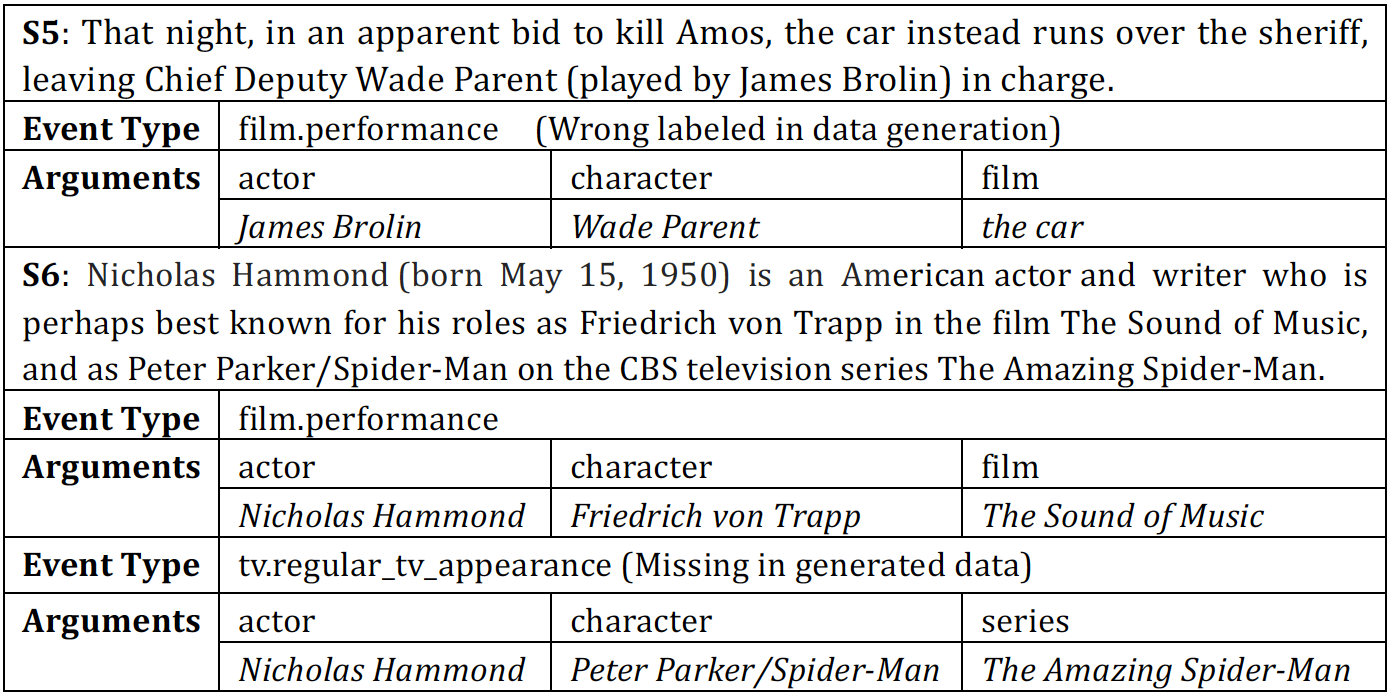
\includegraphics[width=.48\textwidth]{example.png}
	\caption{Example outputs of LSTM-CRF-ILP$_{multi}$.\label{fig:1}}
\end{figure}

Moreover, manual evaluation helps us to gain a deep insight of our data and models. We further conduct automatic evaluation on the manually annotated dataset and list the top 5 event types whose F1 scores of LSTM-CRF-ILP$_{multi}$ differ greatly from automatic evaluation in Table~\ref{tab:4}.

Most of the performance differences are caused by data generation. Figure~\ref{fig:1} examples two types of errors in data generation. Some automatically labeled sentences do not imply any event while still matching all key properties of certain instances. Take S5 as an example. Although the phrase \emph{the car} matches a film name, it does not indicate this film, and there is no explicit evidence expressing that an actor starring in a film. This is a bottleneck of our data generation strategy. During manual evaluation, we find 16 negative sentences which are mistakenly labeled due to this reason. Unfortunately, our model fails to rectify 10 of them.

Remarkably, our LSTM-CRF-ILP$_{multi}$ model can help find more CVT instances that are not referenced in Freebase. There are two events mentioned in S6, while the arguments of the second event do not match any CVT instances in Freebase, leading to a missing event in data generation. This phenomenon suggests that learning from distant supervision provided by Freebase, our model can help complete and update properties of Freebase instances in return.

\begin{table}[h]
\small
\centering
\begin{tabular}{|l|c|c|c|} \hline
	Event type & P & R & F \\ \hline
	olympics.medal\_honor%\footnote{The full name is olympics.olympic\_medal\_honor in Freebase.}
	& $\downarrow$ 25.0\% & $\downarrow$ 5.0\% & $\downarrow$ 13.8\% \\ \hline
	film.performance & $\downarrow$ 21.4\% & $\uparrow$ 3.1\% & $\downarrow$10.3\% \\ \hline
	business.acquisition & $\rightarrow$ & $\downarrow$ 7.1\% & $\downarrow$ 5.4\% \\ \hline
	tv.appearance%\footnote{The full name is tv.regular\_tv\_appearance in Freebase.}
	& $\downarrow$ 9.5\% & $\uparrow$ 3.0\% & $\downarrow$ 3.1\% \\ \hline
	film.release%\footnote{The full name is film.film\_regional\_release\_date in Freebase.}
	& $\downarrow$ 7.7\% & $\uparrow$ 5.6\% & $\downarrow$ 0.55\% \\ \hline
\end{tabular}
\caption{Top 5 event types whose performances on event classification differ most from automatic evaluation. The evaluated model is LSTM-CRF-ILP$_{multi}$ \label{tab:4}}
\end{table}

\subsection{Tables as Supervision}
To demonstrate the applicability of our approach to other structured tables besides Freebase CVT tables, we conduct manual evaluation on a new auto-annotated dataset with supervision provided by large Wikipedia tables. We acquire three tables characterizing events about acquisition, winning the Olympics, and winning the prestigious awards in entertainment industry. To evaluate the performance, we randomly select 100 sentences and follow the same steps of event annotations as mentioned in Section~\ref{manualeve}. 

\begin{table}[h]
\small
\centering
\begin{tabular}{|l|c|c|c|c|c|} \hline
	Event type & Table size & Dataset & EC & AD & ED \\ \hline
	Acquisition & 690 & 414 & 87.0 & 72.0 & 69.6 \\ \hline
	Olympics & 2503 & 1460 & 77.2 & 64.5 & 38.6 \\ \hline
	Awards & 3039 & 2217 & 95.0 & 82.8 & 58.6 \\ \hline
\end{tabular}
\caption{Statistics of the dataset and overall performance of our LSTM-CRF-ILP$_{multi}$ model. \textit{Table size} is the number of table entries. \textit{Dataset} is the size of training set. \label{tab:6}}
\end{table}

Table~\ref{tab:6} demonstrates that our approach with tabular data as distant supervision can be adapted to extract high-confidence events. Given a specific event type, as long as we acquire tables implying events of such type, we can construct a dataset and train an effective event extractor, which is much easier than human annotation and unlimited in event types. 

\section{Related Work}
%Event extraction is one of the fundamental tasks in information extraction. % and natural language understanding. 
Most event extraction works are within the tasks defined by several evaluation frameworks (e.g., MUC~\cite{grishman1996message}, 
ACE~\cite{doddington2004automatic}, ERE~\cite{song2015light} and TAC-KBP~\cite{mitamura2015event}), 
all of which can be considered as a template-filling-based extraction task.
These frameworks focus on limited number of event types, which are designed and annotated by human experts and
hard to generalize to other domains.  
%Most approaches within  these frameworks 
Furthermore, existing extraction systems, which usually adopt a supervised learning paradigm, 
have to rely on those high-quality training data within those frameworks, 
thus hard to move to more domains in practice, regardless of feature-based~\cite{gupta2009predicting,hong2011using,li2013joint} or neural-network-based methods~\cite{chen2015event,nguyen2016joint}.

Besides the works focusing on small human-labeled corpus, 
Huang et al. \shortcite{huang2016liberal}  propose a novel Liberal Event Extraction paradigm 
which automatically discovers event schemas and extract events simultaneously from any unlabeled corpus. 
In contrast, we propose to exploit existing structured knowledge bases, e.g., Freebase, to automatically discover 
types of events as well as their corresponding argument settings, without expert annotation, and further automatically
construct training data, with the essence of distant supervision~\cite{mintz2009distant}.

Distant supervision~(\texttt{DS}) has been widely used in binary relation extraction, where the key assumption is that 
 sentences containing both the subject and object of a $<$$subj$, $rel$, $obj$$>$ triple can be seen as its support, and further
used to train a classifier to identify the relation $rel$. However,  this assumption does not fit to our event extraction scenario, 
where an event usually involves several arguments and it is hard to collect enough training sentences with all arguments appearing in, as indicated by the low coverage of \textbf{H1}. We therefore investigate different hypotheses  for event extraction within the \texttt{DS} paradigm and propose to utilize time and syntactic clues to refine the \texttt{DS} assumption for better data quality. We further relieve the reliance on event trigger annotations by previous event extractors, and define a novel event extraction paradigm with key arguments to characterize an event type. 

 
%
%However, these the reliance on high-quality training data are usually  human-annotated, and  training data prevents  
%
%We typically divide them into feature-based methods and neural-network-based methods. 
%
%Most traditional feature-based methods %usually rely on a variety of elaborate features. They 
% aim to exploit different feature extraction strategies and evaluate their contributions. 
%Besides training classifiers for each subtask, there are also works  jointly learning trigger labeling 
%and argument labeling using structured prediction models to capture both local and global 
%features of triggers and arguments~\cite{li2013joint}. 
%
%Neural-network-based methods are free of hard feature engineering and error propagation from  external NLP tools. 
%In the neural-network side, both convolutional neural network (CNN)~\cite{chen2015event}  and RNN have been employed 
%to extract features of different levels. 
%avoid hard feature engineering and error propagation from  external NLP tools. 
%Two types of neural works have been employed. Chen et al. \shortcite{chen2015event} 
%propose a convolutional neural network (CNN) with a dynamic multi-pooling layer to capture sentence-level features better. 
%Nguyen et al. \shortcite{nguyen2016joint} benefit from  a bidirectional RNN with various memory 
%matrices to jointly learn triggers and arguments within the ACE framework.% which benefits from both joint models and neural network  models. 
%However, to our knowledge, LSTM-CRF models have not been applied in earlier studies.
%
%In contrast to these prior systems focused on small human-labeled corpus, Huang et al. \shortcite{huang2016liberal} 
%propose a novel Liberal Event Extraction paradigm which automatically discovers event schemas and extract events 
%simultaneously from any unlabeled corpus. 

\section{Conclusions and Future Work}
In this paper, we propose a new event extraction paradigm without expert-designed event templates by leveraging structured knowledge bases to automatically acquire event schema and corresponding training data. We propose an LSTM-CRF model with ILP-based post inference to extract events without explicit trigger annotations. Experimental results on both manual and automatic evaluations show that it is possible to learn to extract KB-style events on automatically constructed training data.
Furthermore, our model can extract information not covered by Freebase which indicates the possibility to extend this work to knowledge base population.

% \section*{Acknowledgments}

% Do not number the acknowledgment section.

\bibliography{emnlp2017}
\bibliographystyle{emnlp_natbib}

\end{document}
